\documentclass[class=article,10pt,crop=false]{standalone}
\usepackage{preamble}

\begin{document}
\begin{multicols}{2}[\section{Mecànica i relativitat}]
\subsection{Mecànica}
\subsubsection{Cinemàtica}
Equacions del moviment: $$\Vec{r}(t)=x(t)\Vec{e}_x+y(t)\Vec{e}_y+z(t)\Vec{e}_z$$
Velocitat mitjana: $$\Vec{v}_m=\frac{\Delta\Vec{r}}{\Delta t}$$
Velocitat instantània:
\begin{gather*}
    \Vec{v}(t)=\lim_{\Delta t\to 0}\frac{\Delta\Vec{r}}{\Delta t}=\dot{\Vec{r}}(t)\\
    \dot{\Vec{r}}(t)=\dot{x}(t)\Vec{e}_x+\dot{y}(t)\Vec{e}_y+\dot{z}(t)\Vec{e}_z
\end{gather*}
Celeritat: $v(t)\equiv|\Vec{v}(t)|=|\dot{\Vec{r}}(t)|$\newline
Acceleració mitjana: $$\Vec{a}_m=\frac{\Delta\Vec{v}}{\Delta t}=\frac{\Delta\dot{\Vec{r}}}{\Delta t}$$
Acceleració instantània: 
\begin{gather*}
    \Vec{a}(t)=\lim_{\Delta t\to 0}\frac{\Delta\Vec{v}}{\Delta t}=\ddot{\Vec{r}}(t)\\
    \ddot{\Vec{r}}(t)=\ddot{x}(t)\Vec{e}_x+\ddot{y}(t)\Vec{e}_y+\ddot{z}(t)\Vec{e}_z
\end{gather*}
Moviment rectilini:
\begin{enumerate}
    \item uniforme:
    $$x(t)=x_0+vt$$
    \item uniformement accelerat:
    \begin{gather*}
        x(t)=x_0+v_0t+\frac{1}{2}at^2\\
        \dot{x}(t)=v_0+at
    \end{gather*}
\end{enumerate}
Moviment circular en coordenades polars:
\begin{gather*}
    x=r\cos\varphi\qquad y=r\sin \varphi\\
    \Vec{e}_r=\cos\varphi\Vec{e}_x+\sin\varphi\Vec{e}_y\\
    \Vec{e}_\varphi=-\sin\varphi\Vec{e}_x+\cos\varphi\Vec{e}_y\\
    \Vec{r}=r\Vec{e}_r\quad\Vec{v}=r\omega\Vec{e}_\varphi\quad\Vec{a}=r\alpha\Vec{e}_\varphi-r\omega^2\Vec{e}_r
\end{gather*}
Vectors de Frenet: Eixos de coordenades tangent i normal a la trajectòria en un determinat punt.
\begin{enumerate}
    \item 1r vector de Frenet (tangent):
    $$\Vec{e}_1(t)=\frac{\dot{\Vec{r}}(t)}{|\dot{\Vec{r}}(t)|}$$
    \item 2n vector de Frenet (normal):
    $$\Vec{e}_2(t)=\frac{\dot{\Vec{e}}_1(t)}{|\dot{\Vec{e}}_1(t)|}$$
\end{enumerate}
Celeritat i acceleració:
\begin{gather*}
    \dot{\Vec{r}}(t)=v_t(t)\Vec{e}_1\\
    \ddot{\Vec{r}}(t)=a_t(t)\Vec{e}_1+a_n(t)\Vec{e}_2(t)
\end{gather*}
Curvatura $k$ i radi de curvatura $R$:
$$\frac{1}{k(t)}=R(t)=\frac{|\dot{\Vec{r}}(t)|}{|\dot{\Vec{e}}_1(t)|}$$
Acceleració normal: $$a_n=\frac{v^2}{R}$$ {on $R$ és el radi de curvatura instantani.}\newline
Curvatura mitjana: $$k_m=\frac{\Delta \varphi}{\Delta s}$$
Curvatura: $$k=\lim_{\Delta s\to 0}\frac{\Delta \varphi}{\Delta s}=\frac{d\varphi}{ds}$$
Tir parabòlic:
\begin{gather*}
    x(t)=x_0+v_0\cos\varphi t\\
    y(t)=y_0+v_0\sin\varphi t-\frac{1}{2}gt^2\\
    v_x(t)=v_0\cos\varphi\\
    v_y(t)=v_0\sin\varphi-gt
\end{gather*}
\subsubsection{Dinàmica}
Segona llei de Newton: $$\frac{\Vec{F}(\Vec{r}(t),\dot{\Vec{r}}(t),t)}{m}=\ddot{\Vec{r}}(t)$$
Força gravitatòria: $$\Vec{F}=-G\frac{Mm}{r^2}\hat{r}$$
Força elàstica: $$F_e=-kx$$
Oscil·lador:
\begin{gather*}
    F_e=ma\iff\ddot{x}(t)+\omega^2x(t)=0\\
    x(t)=A\cos(\omega t+\phi)\\
    \dot{x}(t)=-\omega A\sin(\omega t+\phi)\\
    \ddot{x}(t)=-\omega^2 A\cos(\omega t+\phi)=-\omega^2x(t)\\
    \omega=\sqrt{\frac{k}{m}}\qquad T=\frac{2\pi}{\omega}\qquad\nu=\frac{1}{T}
\end{gather*}
Coeficients de fregament:
\begin{itemize}
    \item $\mu_e=$ coeficient estàtic de fregament.
    \item $\mu_c=$ coeficient cinètic de fregament.
\end{itemize} 
Força de fregament: $$F_f=\left\{
    \begin{array}{rcl}
    F & \text{si} & F\leq\mu_eF_{\!_N} \\
    \mu_cF_{\!_N} & \text{si} & F>\mu_eF_{\!_N}
    \end{array}\right.$$
    {on $F$ és la força aplicada a l'objecte i $F_{\!_N}$ la força normal.}\newline
Forces inercials: força fictícia per a sistemes de referència no inercials. $$\Vec{F}(t)+\Vec{F}_{\text{iner}}(t)=m\ddot{\Vec{r}}\,'(t)$$ {on $\Vec{F}_{\text{iner}}(t)\equiv-m\ddot{\Vec{R}}(t)$ i $\Vec{R}(t)$ és l'equació del moviment d'un sistema de referència respecte de l'altre.}\newline
Transformacions de Galileo:
\begin{align*}
    x'&=x-Vt & v_x'&=v_x-V\\
    y'&=y & v_y'&=v_y\\
    z'&=z & v_z'&=v_z\\
    t'&=t
\end{align*} {on $V$ és la velocitat de $S'$ respecte $S$.}
\subsubsection{Estàtica}
Moment lineal: $$\Vec{p}=mv$$
Segona llei de Newton: $$\Vec{f}=\frac{d\Vec{p}}{dt}$$
Moment lineal del sistema:
\begin{gather*}
    \Vec{P}=\sum_i\Vec{p}_{Oi}\\
    \frac{d\Vec{P}}{dt}=\Vec{F}_\text{total}^\text{ext}
\end{gather*}
Centre de masses: 
\begin{gather*}
\Vec{R}=\frac{\sum_im_i\Vec{r}_i}{M}\\
M\dot{\Vec{R}}=\sum_im_i\Vec{v}_i=\Vec{P}\\
M\ddot{\Vec{R}}=\frac{d\Vec{P}}{dt}=\Vec{F}_\text{total}^\text{ext}
\end{gather*}{on $M=\sum_i m_i$.}\newline
Centre de masses d'un sòlid rígid: $$\Vec{R}=\frac{1}{M}\int_V\Vec{r}\rho dV$$ {on $M=\int_V\rho dV$.}\newline
Moment angular: $$\Vec{l}_O=\Vec{r}\times\Vec{p}$$
Moment angular del sistema: $$\Vec{L}_O=\sum_i\Vec{l}_{Oi}$$
Moment d'una força: $$\Vec{m}_O=\Vec{r}\times\Vec{f}$$
Moment de les forces: 
\begin{gather*}
    \Vec{M}_O=\sum_i\Vec{m}_{Oi}\\
\dot{\Vec{l}}_O=\Vec{m}_O\qquad\dot{\Vec{L}}_O=\Vec{M}_O^\text{ext}
\end{gather*}
Conservació del moment angular: $$\Vec{M}_O^\text{ext}=0\implies\frac{d\Vec{L}_O}{dt}=0$$
Sòlids en equilibri estàtic: $$\Vec{F}_\text{total}^\text{ext}=0\qquad\Vec{M}_O^\text{ext}=0$$
\subsubsection{Treball i energia}
Treball: \begin{gather*}
    W=\Vec{F}\cdot\Delta\Vec{r}=F\Delta r\cos\theta\\
    W=\lim_{N\to\infty}\sum_{i=1}^N\Vec{F}_i\cdot\Delta\Vec{r}_i=\int_C\Vec{F}\cdot\text{d}\Vec{r}
\end{gather*}
Potència: $$P=\frac{W}{\Delta t}$$
Energia cinètica: $$K=\frac{1}{2}mv^2$$
Teorema treball-energia cinètica:
$$W=\Delta K$$
Potència instantània: $$P=\Vec{F}\cdot\Vec{v}$$
Energia potencial elàstica: $$U=\frac{1}{2}kx^2$$
Treball de forces conservatives: $$W=-\Delta U$$
Energia mecànica: $$E=K+U$$
\begin{itemize}
    \item Si actuen només forces conservatives: $$\Delta E=0$$
    \item Si hi ha forces no conservatives: $$\Delta E=W_{\text{nc}}$$ {on $W_\text{nc}$ és el treball fet per les forces no conservatives.}
\end{itemize}
Energia potencial gravitatòria: 
\begin{itemize}
    \item Per a alçades petites $h$ sobre la superfície de la terra:$$U=mgh$$
    \item Per al cas general:$$U=-\frac{GMm}{r}$$
\end{itemize}
Velocitat d'escapament: $$v=\sqrt{\frac{2GM}{R}}$$
\subsubsection{Rotació}
Moment d'inèrcia: $$I_e=\sum_im_i\eta_i^2$$ {on $\eta_i$ és la distància entre la posició de la partícula de massa $m_i$ i l'eix $e$.}\newline
Moment angular: $$L_e=I_e\omega$$
Sòlid rígid: $$M_e^\text{ext}=\dot{L}_e=I_e\dot{\omega}=I_e\alpha$$
Moment angular respecte del CM:$$\Vec{L}_O=\Vec{L}_{CM}+\Vec{R}\times\Vec{P}$$ {on $\Vec{R}$ és la distància del $CM$ al punt $O$.}\newline
Moment d'una força respecte del CM: $$\Vec{M}_O^\text{ext}=\Vec{M}_{CM}^\text{ext}+\Vec{R}\times\Vec{F}_\text{total}^\text{ext}$$ {on $\Vec{R}$ és la distància del $CM$ al punt $O$.}
$$\dot{\Vec{L}}_{CM}=\Vec{M}_{CM}^\text{ext}$$
Energia cinètica de rotació: $$K=\frac{1}{2}MV^2+\frac{1}{2}I_{CM}\omega^2$$
Teorema d'Steiner: $$I_{e'}=I_e+Ma^2$$ {on $a$ és la distància entre els eixos $e$ i $e'$.}
\subsection{Relativitat}
Factor de Lorentz:
$$\gamma=\frac{1}{\sqrt{1-\beta^2}}$$ {on $\beta=v/c$.}\newline
Transformacions de Lorentz:
\begin{align*}
    x'&=\gamma(x-\beta ct) & x&=\gamma(x'+\beta ct')\\
    y'&=y & y&=y'\\
    z'&=z & z&=z'\\
    ct'&=\gamma(ct-\beta x) & ct&=\gamma(ct'+\beta x')
\end{align*}
{on $v$ és la velocitat de $S'$ respecte de $S$.}\newline
Dilatació temporal:
$$\Delta t=\gamma \Delta t_0^{}$$ {on $\Delta t_0^{}$ és el temps propi, és a dir, el temps mesurat entre dos esdeveniments per un sistema de referència on aquests dos succeeixen al mateix lloc.}\newline
Contracció de longituds:
$$\Delta l=\frac{\Delta l_0^{}}{\gamma}$$ {on $\Delta l_0^{}$ és la longitud pròpia, és a dir, és la longitud mesurada en un sistema de referència on l'objecte està en repòs.}\newline
Invariant de Lorentz:
$$s^2=c^2t^2-x^2-y^2-z^2$$
\begin{itemize}
    \item $s^2>0\implies\textit{timelike}$
    \item $s^2=0\implies\textit{lightlike}$
    \item $s^2<0\implies\textit{spacelike}$
\end{itemize}
Els esdeveniments \textit{timelike} i \textit{lightlike} estan en contacte causal amb l'origen (és possible enviar un senyal de llum des del punt a l'origen o viceversa), mentre que els \textit{spacelike} no.\newline
\begin{figure}[ht]
    \centering
    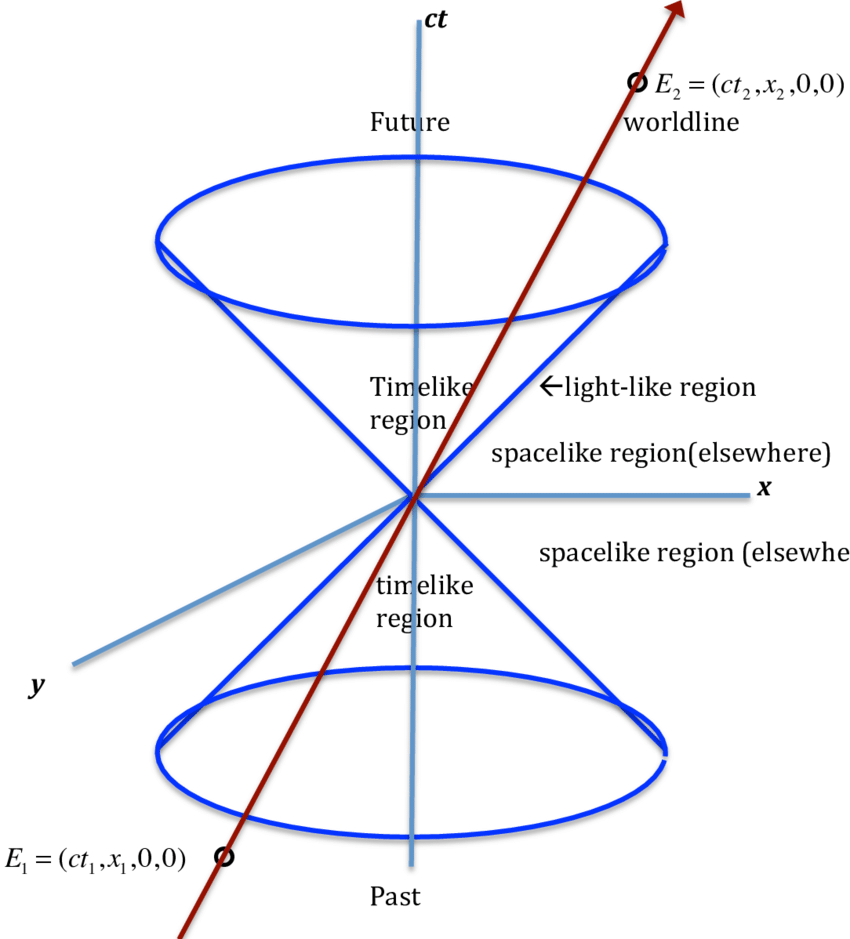
\includegraphics[width=4cm]{Physics/1st/Mecanica_i_relativitat/Imatges/mink.png}
    \caption{Con del passat i del futur.}
\end{figure}
Transformacions de Lorentz (velocitats):
\begin{align*}
    u_x'&=\frac{u_x-v}{1-u_xv/c^2} & u_x&=\frac{u_x'+v}{1+u_x'v/c^2}\\
    u_y'&=\frac{u_y}{\gamma \left(1-u_xv/c^2\right)} & u_y&=\frac{u_y'}{\gamma \left(1+u_xv/c^2\right)}\\
    u_z'&=\frac{u_z}{\gamma \left(1-u_xv/c^2\right)} & u_z&=\frac{u_z'}{\gamma \left(1+u_xv/c^2\right)}
\end{align*}
Efecte Doppler:
$$\nu_{\!_R}=\frac{\nu_{\!_E}}{\gamma(1-\beta\cos\phi)}$$
{on $\phi$ és l'angle, respecte del receptor, entre la ve\-lo\-ci\-tat de la font i la direcció de la llum i $\nu_{\!_E}$ i $\nu_{\!_R}$ són les freqüències de l'emissor i el receptor, respectivament.}\newline
\begin{figure}[ht]
    \centering
    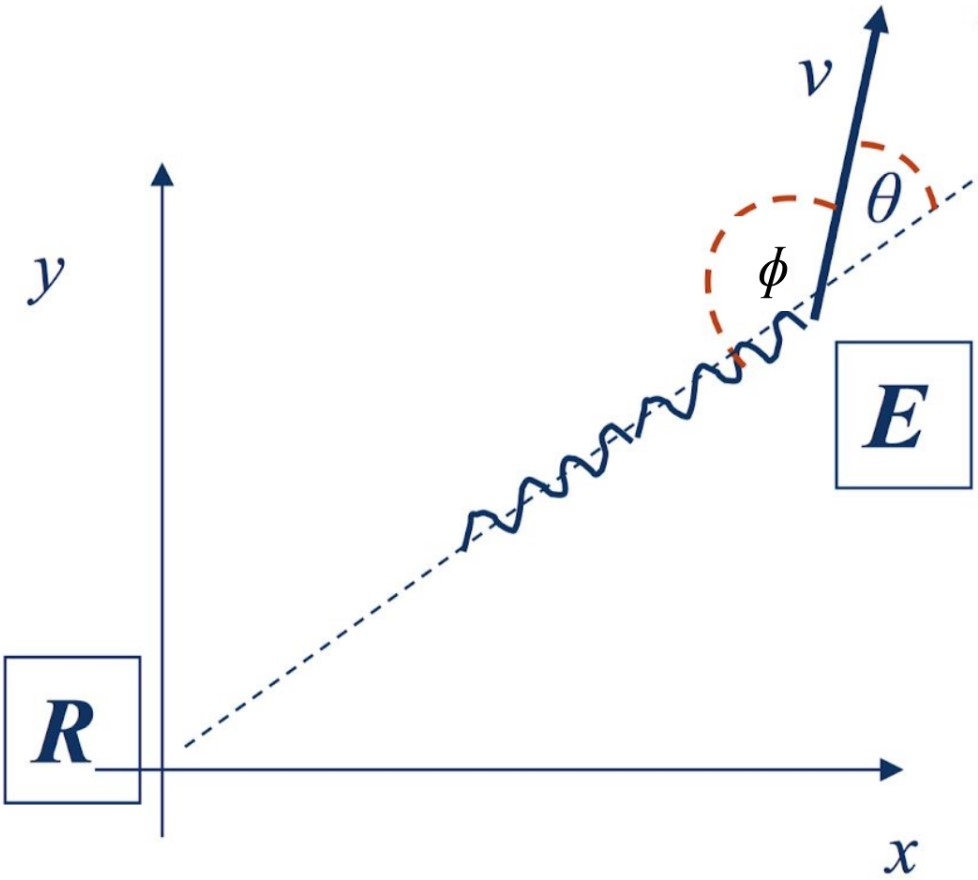
\includegraphics[width=4cm]{Physics/1st/Mecanica_i_relativitat/Imatges/dop.jpg}
    \caption{Cas general d'efecte Doppler relativista.}
\end{figure}
$$\tan\frac{\phi'}{2}=\sqrt{\frac{1+\beta}{1-\beta}}\tan\frac{\phi}{2}$$
{on $\phi'$ és l'angle, respecte de l'emissor, entre la velocitat de la font i la direcció de la llum.} \newline
Efecte Doppler longitudinal:
\begin{itemize}
    \item Si la font s'allunya ($\phi=\pi$):
   $$\nu_{\!_R}=\nu_{\!_E}\sqrt{\frac{1-\beta}{1+\beta}}$$
   \item Si la font s'apropa ($\phi=0$):
   $$\nu_{\!_R}=\nu_{\!_E}\sqrt{\frac{1+\beta}{1-\beta}}$$
\end{itemize}
Efecte Doppler transversal ($\phi=\pi/2$):
$$\nu_{\!_R}=\nu_{\!_E}/\gamma$$
Energia relativista:
$$E=\gamma mc^2=\sqrt{p^2c^2+m^2c^4}$$
Moment relativista:
$$\vec{p}=\gamma m\vec{u}$$
Massa relativista:
$$m_r=\gamma m$$ {on $m$ és la massa, invariant, de l'objecte en repòs.}\newline
Energia i moment dels fotons:
$$E=h\nu\qquad E=|\vec{p}|c$$
Transformacions de Lorentz (Energia $-$ moment):
\begin{align*}
    E'&=\gamma(E-\beta cp_x) & E&=\gamma(E'+\beta cp_x')\\
    cp_x'&=\gamma(cp_x-\beta E) & cp_x&=\gamma(cp_x'+\beta E')\\
    p_y'&=p_y & p_y&=p_y'\\
    p_z'&=p_z & p_z&=p_z'
\end{align*}
Efecte Compton:
$$\lambda'-\lambda=\frac{h}{mc}(1-\cos\theta)$$
{on $\lambda$ i $\lambda'$ són les longituds d'ona dels fotons abans i després de dispersió, $\theta$ és l'angle de dispersió, $m$ és la massa de la partícula en repòs i $\lambda_c=\frac{h}{mc}$ és la longitud d'ona Compton.}\newline 
\begin{figure}[ht]
    \centering
    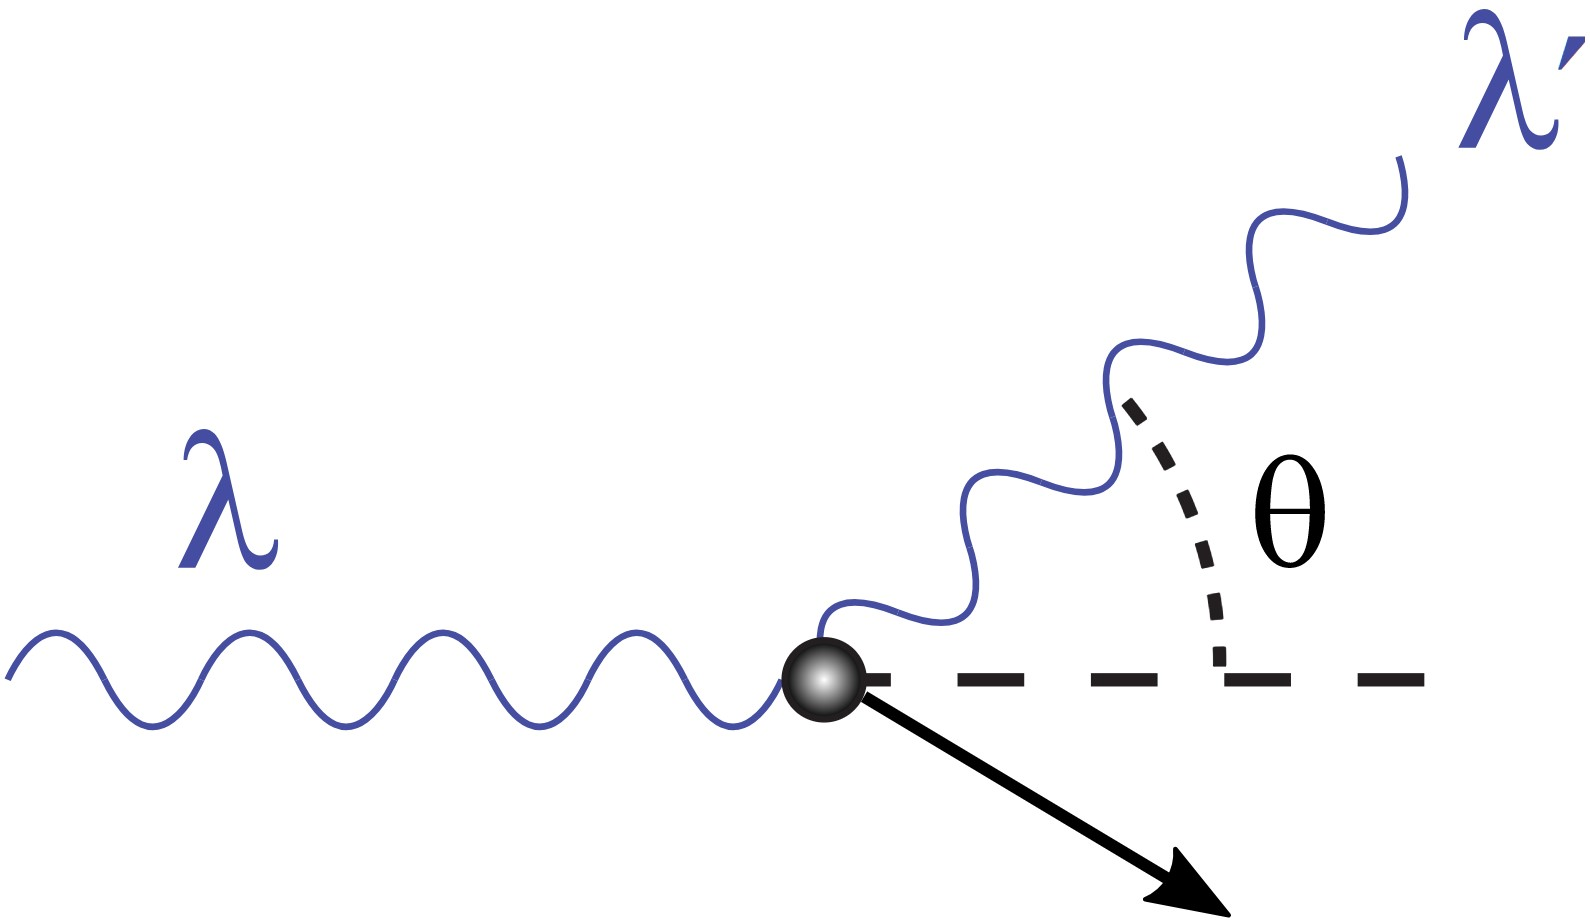
\includegraphics[width=4cm]{Physics/1st/Mecanica_i_relativitat/Imatges/comp.jpg}
    \caption{Efecte Compton. Normalment la par\-tí\-cu\-la de massa sol ser un electró.}
\end{figure}
\subsection{Fluids}
Pressió en un punt $p(x)$ (considerant una esfera molt petita al voltant del punt $x$):
$$p(x)=\frac{\sum F_{\!_N}}{S}$$
Pressió hidrostàtica:
$$p=p_{\!_0}+\rho g\Delta h$$
{on $p_{\!_0}$ és la pressió a un punt a una distància vertical $\Delta h$ del punt on hi ha una pressió $p$.}\newline
Principi de Pascal:
$$p_{\!_1}=\frac{F_{\!_1}}{S_{\!_1}}=\frac{F_{\!_2}}{S_{\!_2}}=p_{\!_2}$$
Principi d'Arquímedes (empenta hi\-dros\-tà\-ti\-ca):
$$F_{\!_E}=m_{\!_L}g=\rho_{\!_L}Vg$$
{on $m_{\!_L}$ i $V$ són respectivament la massa i el volum de líquid desallotjat.}\newline
Equació de la continuïtat (per a fluids incompressibles):
$$Q_{\!_1}=S_{\!_1}v_{\!_1}=S_{\!_2}v_{\!_2}=Q_{\!_2}$$ {on $Q_i$ és el cabal; $S_i$, la secció, i $v_i$, la velocitat en l'instant $i$.}\newline
Principi de Bernoulli (per a fluids incompressibles, sense viscositat i amb flux laminar i estacionari):
$$p+\rho gh+\frac{1}{2}\rho v^2=\text{constant}$$
Força de sustentació:
$$F_{\!_L}=\frac{1}{2}C_{\!_L}\rho Sv^2$$
{on $C_{\!_L}$ és el coeficient de sustentació.}\newline
Velocitat mínima de sustentació:
$$v_{\text{min}}=\sqrt{\frac{2mg}{C_{\!_L}\rho S}}$$
Viscositat:\newline
\begin{figure}[ht]
    \centering
    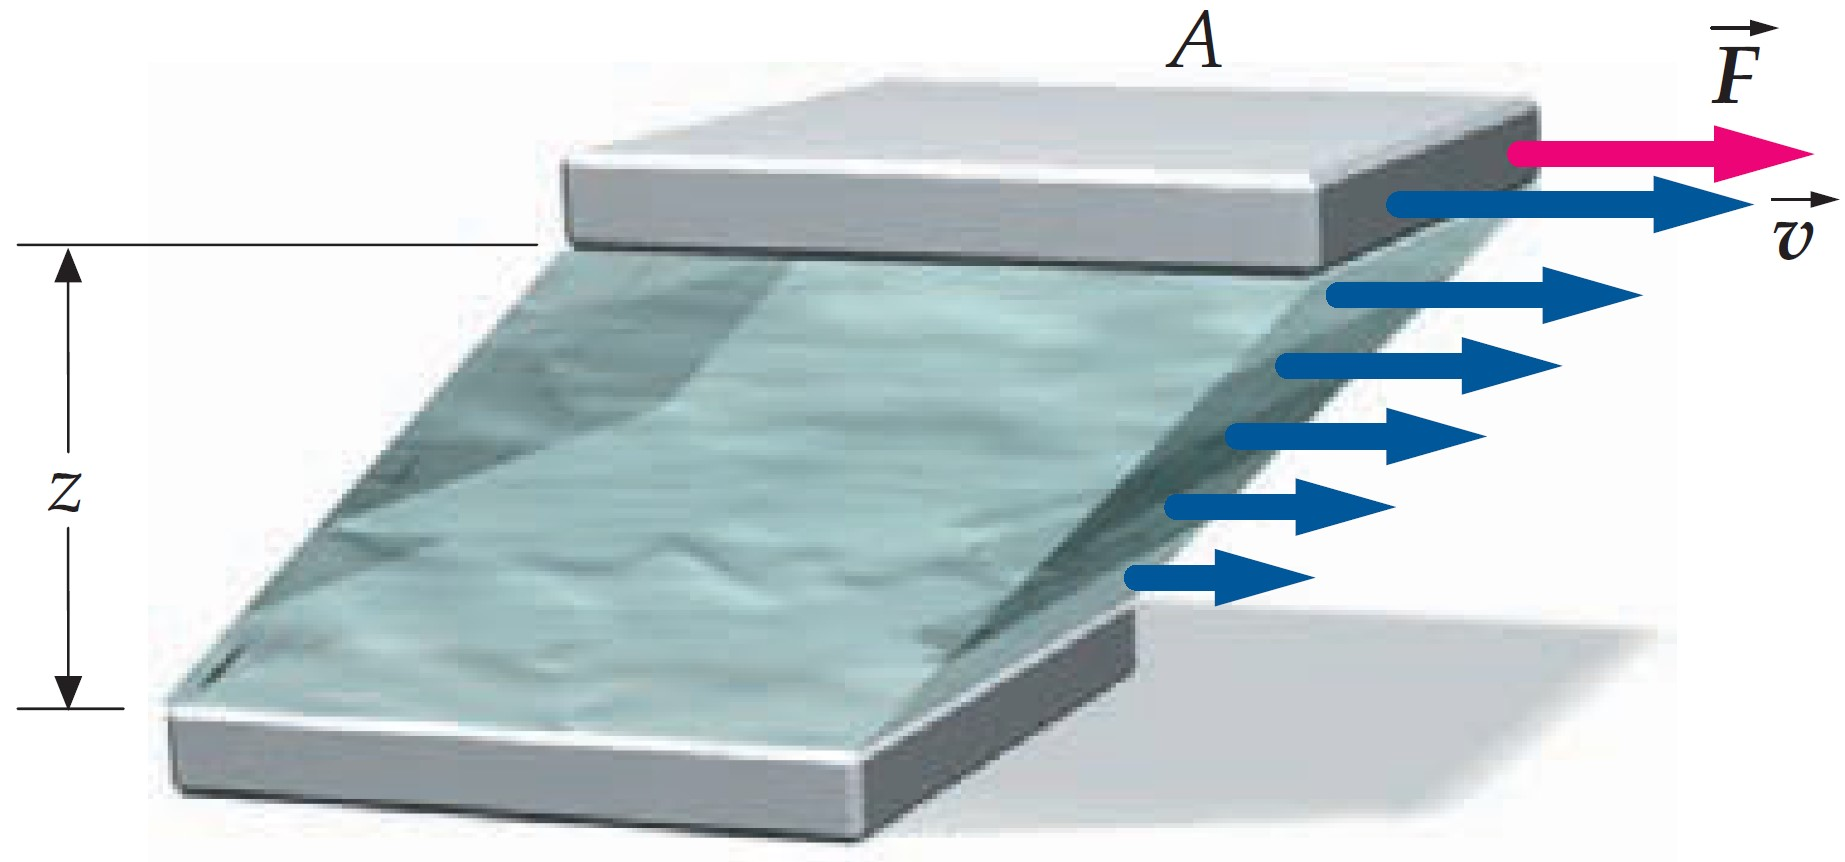
\includegraphics[width=4cm]{Physics/1st/Mecanica_i_relativitat/Imatges/vis.jpg}
    \caption{Força de viscositat.}
\end{figure}
$$F=\eta\frac{vA}{z}$$
{on $F$ és la força actuant a la tapa de dalt (d'àrea $A$) separada una distància $z$ de l'altra tapa per un fluid de viscositat $\eta$ movent-se a velocitat $v$.}\newline
Velocitat en un canal:\newline
\begin{figure}[ht]
    \centering
    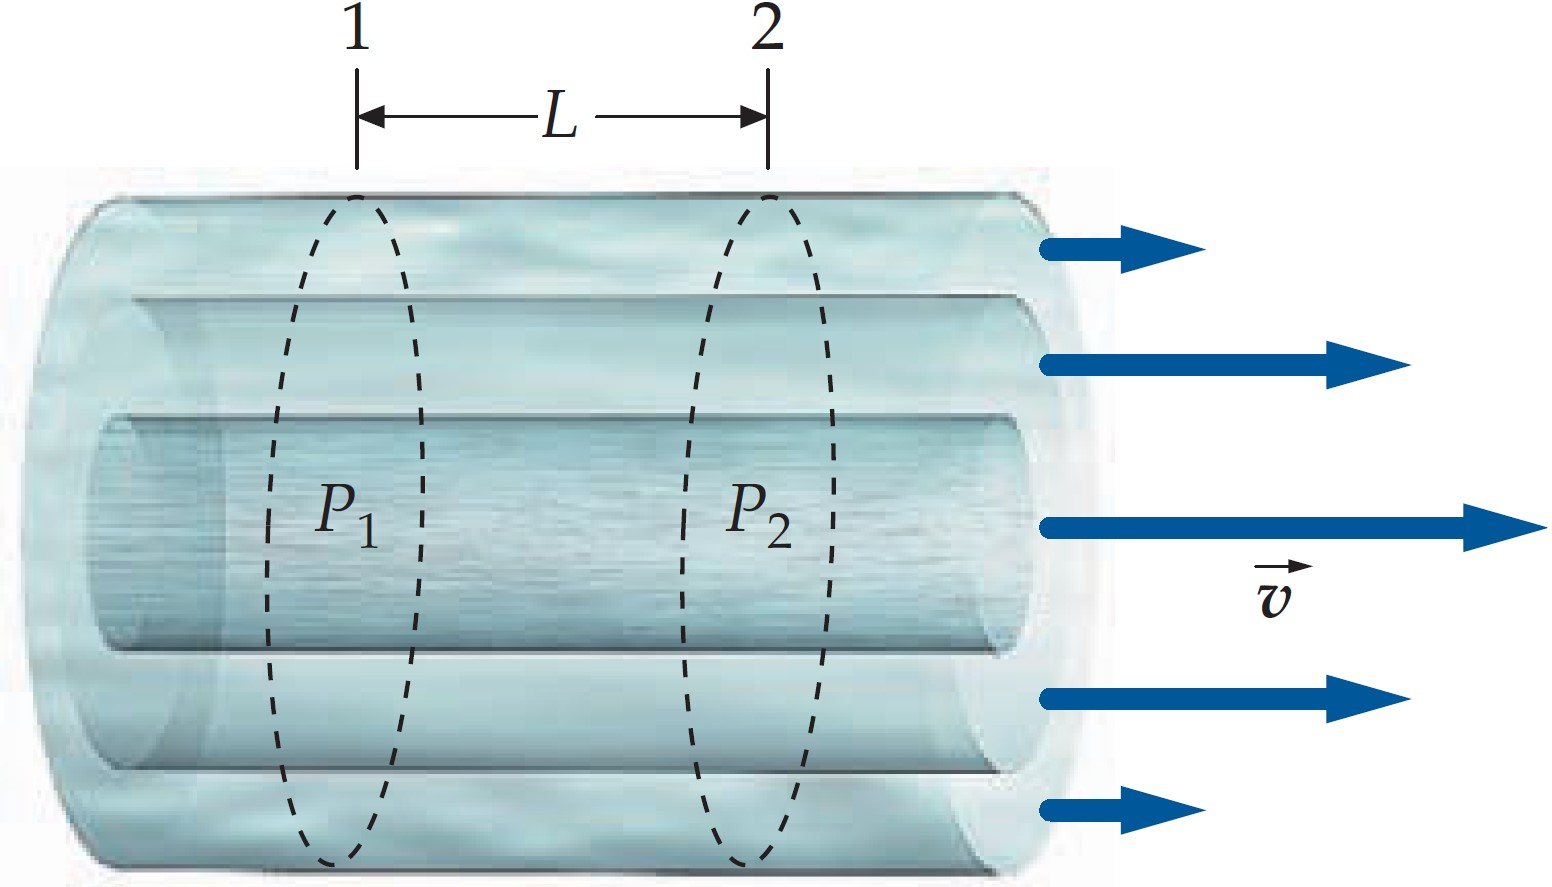
\includegraphics[width=4cm]{Physics/1st/Mecanica_i_relativitat/Imatges/vis2.jpg}
    \caption{Velocitat en un fluid amb viscositat $\eta$.}
\end{figure}
$$v(x)=\frac{\Delta p}{4\eta L}(r^2-x^2)$$
$$\langle v\rangle=\frac{\Delta p}{8\eta L}r^2$$
{on $v(x)$ és la velocitat del fluid a un punt $x$ per sobre l'eix del canal entre dos punts separats una distància $L$ amb diferència de pressió $\Delta p=p_1-p_2$. $\langle v\rangle=v_{\text{max}}/2$ és la velocitat mitjana.}\newline
Llei de Poiseuille:
$$Q=S\langle v\rangle\implies Q=\frac{\pi}{8\eta}\frac{\Delta p}{L}r^4,$$ $$\Delta p=\frac{8\eta}{\pi}\frac{L}{r^4}Q\implies \Delta p=R_f Q$$
{on $R_f:=\frac{8\eta}{\pi}\frac{L}{r^4}$ és la resistència hidrodinàmica. Observem que l'última expressió és anàloga a la llei d'Ohm per a circuits elèctrics.} \newline
Resistències de fluids:
\begin{itemize}
    \item en sèrie: $$R_{\!_T}=\sum_{i=1}^nR_i$$
    \item en paral·lel: $$\frac{1}{R_{\!_T}}=\sum_{i=1}^n\frac{1}{R_i}$$
\end{itemize}
Potència dissipada: $$P=\Delta pQ=R_fQ^2$$
Forces de fregament (viscoses i d'inèrcia):
\begin{itemize}
    \item Velocitats baixes i viscositat alta:\par 
    $$F=k\eta vr$$
    {on $k=6\pi$ si és una esfera i $r$ el radi.}
    \item Velocitats altes i viscositat baixa:
    $$F=\frac{1}{2}C_{\!_a}\rho Sv^2$$
    {on $C_a$ és el coeficient aerodinàmic.}
\end{itemize}
Velocitat límit: \begin{itemize}
    \item Forces viscoses: $$v_{\!_L}=\frac{mg}{k\eta r}$$
    \item Forces d'inèrcia: $$v_{\!_L}=\sqrt{\frac{2mg}{C_a\rho S}}$$
\end{itemize}
Nombre de Reynolds: quantitat adimensional que dona informació sobre el tipus de règim (laminar o turbulent).
$$R_e=\frac{\rho vD}{\eta}\approx\frac{F_{\text{inèrcia}}}{F_{\text{vicosa}}}$$
{on $D$ és el diàmetre.}
$$R_e<2000\implies\text{flux laminar}$$
$$R_e>3000\implies\text{flux turbulent}$$
\end{multicols}
\end{document}